% Options for packages loaded elsewhere
\PassOptionsToPackage{unicode}{hyperref}
\PassOptionsToPackage{hyphens}{url}
%
\documentclass[
  11pt,
  a4paper,
]{article}
\usepackage{amsmath,amssymb}
\usepackage{lmodern}
\usepackage{iftex}
\ifPDFTeX
  \usepackage[T1]{fontenc}
  \usepackage[utf8]{inputenc}
  \usepackage{textcomp} % provide euro and other symbols
\else % if luatex or xetex
  \ifXeTeX
    \usepackage{zxjatype} 
    \usepackage[ipaex]{zxjafont}
    \setromanfont{Times New Roman}
  \fi
  \usepackage{unicode-math}
  \defaultfontfeatures{Scale=MatchLowercase}
  \defaultfontfeatures[\rmfamily]{Ligatures=TeX,Scale=1}
\fi
% Use upquote if available, for straight quotes in verbatim environments
\IfFileExists{upquote.sty}{\usepackage{upquote}}{}
\IfFileExists{microtype.sty}{% use microtype if available
  \usepackage[]{microtype}
  \UseMicrotypeSet[protrusion]{basicmath} % disable protrusion for tt fonts
}{}
\usepackage{xcolor}
\IfFileExists{xurl.sty}{\usepackage{xurl}}{} % add URL line breaks if available
\IfFileExists{bookmark.sty}{\usepackage{bookmark}}{\usepackage{hyperref}}
\hypersetup{
  pdftitle={Draft of Data and Estimation Result},
  hidelinks,
  pdfcreator={LaTeX via pandoc}}
\urlstyle{same} % disable monospaced font for URLs
\usepackage[left=3cm,right=3cm,top=3cm,bottom=3cm]{geometry}

\usepackage{setspace}
\renewcommand{\baselinestretch}{1.5}
\usepackage{float}

\usepackage{longtable,booktabs,array}
\usepackage{threeparttable, threeparttablex, multirow}
\usepackage{calc} % for calculating minipage widths
% Correct order of tables after \paragraph or \subparagraph
\usepackage{etoolbox}
\makeatletter
\patchcmd\longtable{\par}{\if@noskipsec\mbox{}\fi\par}{}{}
\makeatother
% Allow footnotes in longtable head/foot
\IfFileExists{footnotehyper.sty}{\usepackage{footnotehyper}}{\usepackage{footnote}}
\makesavenoteenv{longtable}
\usepackage{graphicx}
\makeatletter
\def\maxwidth{\ifdim\Gin@nat@width>\linewidth\linewidth\else\Gin@nat@width\fi}
\def\maxheight{\ifdim\Gin@nat@height>\textheight\textheight\else\Gin@nat@height\fi}
\makeatother
% Scale images if necessary, so that they will not overflow the page
% margins by default, and it is still possible to overwrite the defaults
% using explicit options in \includegraphics[width, height, ...]{}
\setkeys{Gin}{width=\maxwidth,height=\maxheight,keepaspectratio}
% Set default figure placement to htbp
\makeatletter
\def\fps@figure{htbp}
\makeatother
\setlength{\emergencystretch}{3em} % prevent overfull lines
\providecommand{\tightlist}{%
  \setlength{\itemsep}{0pt}\setlength{\parskip}{0pt}}
\setcounter{secnumdepth}{5}
\newlength{\cslhangindent}
\setlength{\cslhangindent}{1.5em}
\newlength{\csllabelwidth}
\setlength{\csllabelwidth}{3em}
\newlength{\cslentryspacingunit} % times entry-spacing
\setlength{\cslentryspacingunit}{\parskip}
\newenvironment{CSLReferences}[2] % #1 hanging-ident, #2 entry spacing
 {% don't indent paragraphs
  \setlength{\parindent}{0pt}
  % turn on hanging indent if param 1 is 1
  \ifodd #1
  \let\oldpar\par
  \def\par{\hangindent=\cslhangindent\oldpar}
  \fi
  % set entry spacing
  \setlength{\parskip}{#2\cslentryspacingunit}
 }%
 {}
\usepackage{calc}
\newcommand{\CSLBlock}[1]{#1\hfill\break}
\newcommand{\CSLLeftMargin}[1]{\parbox[t]{\csllabelwidth}{#1}}
\newcommand{\CSLRightInline}[1]{\parbox[t]{\linewidth - \csllabelwidth}{#1}\break}
\newcommand{\CSLIndent}[1]{\hspace{\cslhangindent}#1}


\usepackage{booktabs}
\usepackage{siunitx}
\newcolumntype{d}{S[input-symbols = ()]}
\ifLuaTeX
  \usepackage{selnolig}  % disable illegal ligatures
\fi

\makeatletter
\def\@fnsymbol#1{\ensuremath{\ifcase#1\or \dagger\or \ddagger\or
   \mathsection\or \mathparagraph\or \|\or **\or \dagger\dagger
   \or \ddagger\ddagger \else\@ctrerr\fi}}
    \makeatother
\title{Draft of Data and Estimation Result  }
\author{
    Hiroki Kato
  \thanks{Graduate School of Economics, Osaka University, Japan. E-mail: vge008kh@stundent.econ.osaka-u.ac.jp  }
  \and
    Tsuyoshi Goto
  \thanks{Graduate School of Social Sciences, Chiba University, Japan. E-mail: t.goto@chiba-u.jp  }
  \and
    Youngrok Kim
  \thanks{Graduate School of Economics, Kobe University, Japan.  }
  \and
  }

\date{2022/02/17}


\begin{document}
\begin{spacing}{1}
  \maketitle
\end{spacing}

\hypertarget{nastab}{%
\section{National Survey of Tax and Benefit (NaSTaB)}\label{nastab}}

本研究は2008年からKorea Institute of Taxation and Financeが実施した
National Survey of Tax and Benefit (NaSTaB)を用いる。
これは家計の税負担や公的扶助などに関する年次パネルデータである。
この調査は全国から5,634世帯を対象とし、
5,634人の世帯主と15歳以上で経済活動をしている世帯員が調査に回答する。
この調査は前年の所得や寄付額に関する情報を含んでおり、
それらに加えて、教育年数などの個人属性や税制に対する個人の意識に関する情報を含んでいる。

\begin{table}

\caption{\label{tab:SummaryCovariate}Descriptive Statistics}
\centering
\fontsize{9}{11}\selectfont
\begin{tabular}[t]{lcccccc}
\toprule
  & N & Mean & Std.Dev. & Min & Median & Max\\
\midrule
\addlinespace[0.3em]
\multicolumn{7}{l}{\textbf{Income and giving price}}\\
\hspace{1em}Annual taxable labor income (unit: 10,000KRW) & 36189 & \num{1747.26} & \num{2696.77} & \num{0.00} & \num{0.00} & \num{50000.00}\\
\hspace{1em}First giving relative price & 36198 & \num{0.86} & \num{0.04} & \num{0.62} & \num{0.85} & \num{0.94}\\
\addlinespace[0.3em]
\multicolumn{7}{l}{\textbf{Charitable giving}}\\
\hspace{1em}Annual chariatable giving (unit: 10,000KRW) & 36199 & \num{35.64} & \num{153.20} & \num{0.00} & \num{0.00} & \num{10000.00}\\
\hspace{1em}Dummary of donation > 0 & 36199 & \num{0.24} & \num{0.42} & \num{0.00} & \num{0.00} & \num{1.00}\\
\hspace{1em}Dummy of declaration of a tax relief & 36199 & \num{0.10} & \num{0.30} & \num{0.00} & \num{0.00} & \num{1.00}\\
\addlinespace[0.3em]
\multicolumn{7}{l}{\textbf{Individual Characteristics}}\\
\hspace{1em}Age & 36199 & \num{53.45} & \num{16.22} & \num{24.00} & \num{51.00} & \num{103.00}\\
\hspace{1em}Female dummy & 36199 & \num{0.43} & \num{0.50} & \num{0.00} & \num{0.00} & \num{1.00}\\
\hspace{1em}University graduate & 36198 & \num{0.42} & \num{0.49} & \num{0.00} & \num{0.00} & \num{1.00}\\
\hspace{1em}High school graduate dummy & 36198 & \num{0.31} & \num{0.46} & \num{0.00} & \num{0.00} & \num{1.00}\\
\hspace{1em}Junior high school graduate dummy & 36198 & \num{0.27} & \num{0.44} & \num{0.00} & \num{0.00} & \num{1.00}\\
\hspace{1em}Wage earner dummy & 27394 & \num{0.56} & \num{0.50} & \num{0.00} & \num{1.00} & \num{1.00}\\
\bottomrule
\end{tabular}
\end{table}

我々の研究では(1)2013年から2018年かつ、(2)23歳以下の回答者を除いたデータを使用する。
データの期間を制限した理由は、2014年の制度改革に注目するためである。
所得控除制度が適用されている期間(2014年の制度改革前)では、所得税率の改正が寄付行動に影響を与える。
この制度が適用されている期間において、所得税率の改正は2011年が最後である。
したがって、2011年以前の寄付行動を用いると、2014年の制度改革以外の影響を含んでしまう。
その可能性を取り除くために、我々は2013年から2018年のデータ(2012年から2017年の寄付行動)を用いる。
また、23歳以下の回答者を除いた理由は、所得や資産を十分に持っていない可能性が高いからである。
表\ref{tab:SummaryCovariate}に記述統計を示した。

\begin{figure}[t]

{\centering 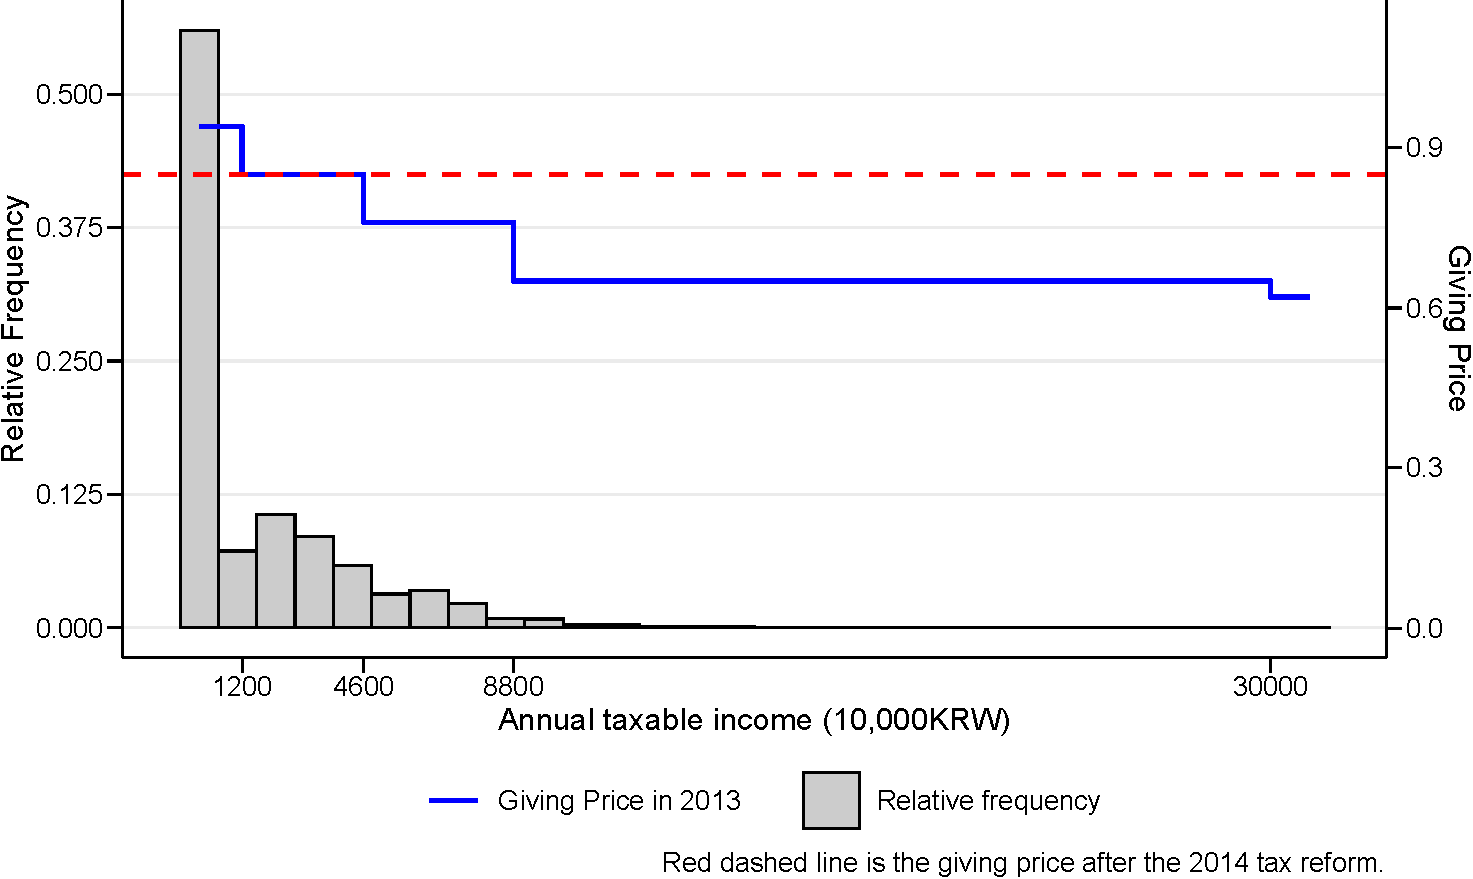
\includegraphics{C:/Users/vge00/Desktop/NASTAB/paper/draft_files/figure-latex/SummaryPrice-1} 

}

\caption{Income Distribution in 2013 and Relative Giving Price. Notes: The left and right axis measure the relative frequency of respondents (grey bars) and the relative giving price (solid step line and dashed line), respectively. A solid step line and a dashed horizontal line represents the giving price in 2013 and 2014, respectively.}\label{fig:SummaryPrice}
\end{figure}

NaSTabは前年の労働所得を調査している。
表\ref{tab:SummaryCovariate}は、
我々が用いるサンプルの労働所得の平均額は17.54 million KRWであることを示しており、
Korean National Tax Serviceが発行しているNational Tax Statistical Yearbook 2012-2018
の平均所得32.77 million KRWより低い。
これはNaSTaBが主婦などの労働所得がない人を含んでいるからである。
したがって、所得分布は右歪曲な分布になる(図\ref{fig:SummaryPrice})。
我々は労働所得に基づいて限界税率を計算し、所得控除における寄付価格を計算した。
図\ref{fig:SummaryPrice}の黒の実線は2012年から2013年の寄付の相対価格を示している。

また、図\ref{fig:SummaryPrice}は価格弾力性を識別するための価格変動も示している。
先に述べたように、黒の実線は所得控除が適用されている期間(2012年から2013年)の寄付の相対価格を示している。
対して、黒の破線は税額控除が適用されている期間(2014年以降)の寄付の相対価格を示している。
2014年の税制改革による税インセンティブの変化に基づいて、我々は三つの所得グループを作ることができる:
(1) 120 million KRWより低い;
(2) 120 million KRWから460 million KRWの間;
(3) 460 million KRWより高い。
第一のグループに属する人の税インセンティブは税制改革によって拡大した(寄付価格が減少した)。
第二のグループに属する人の税インセンティブは税制改革によって変化しなかった。
第三のグループに属する人の税インセンティブは税制改革によって縮小した(寄付価格が増加した)。
このグループによる差分の差分法が我々の第一の識別戦略となる\footnote{2011年以前の寄付行動は所得税率の改正による影響をうけるので、税制改革前の平行トレンドを検証することはできない。}。

\begin{figure}[t]

{\centering 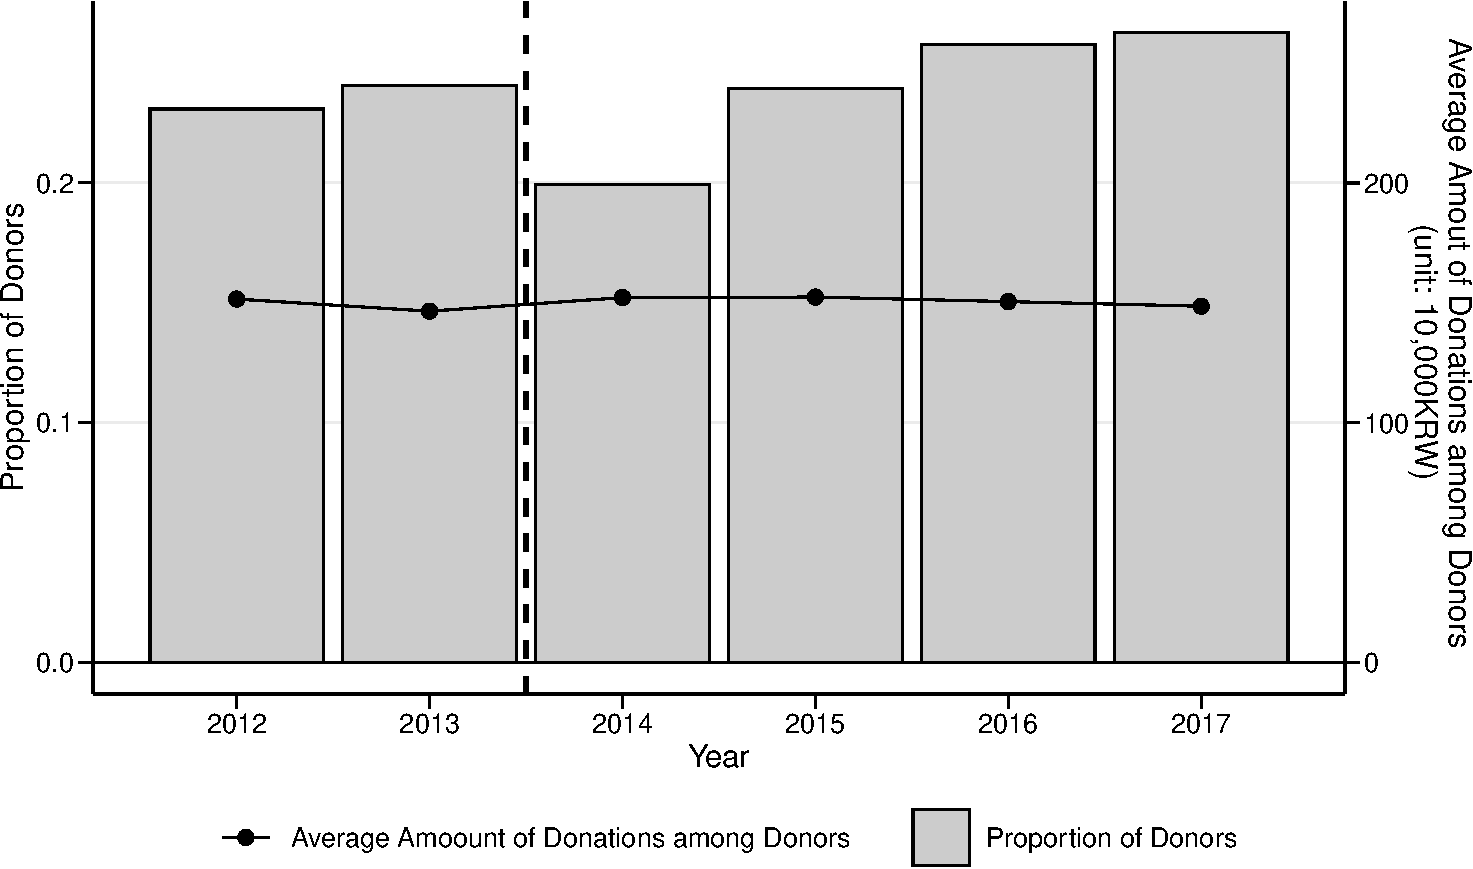
\includegraphics{C:/Users/vge00/Desktop/NASTAB/paper/draft_files/figure-latex/SummaryGiving-1} 

}

\caption{Proportion of Donors and Average Donations among Donors. Notes: The left and right axises measure prooortion of donors (grey bars) and the average amount of donations among donors (solid line), respectively.}\label{fig:SummaryGiving}
\end{figure}

各所得グループの寄付のトレンドを確認する前に、
全体的な寄付行動の傾向を図\ref{fig:SummaryGiving}に示した。
2012年から2017年にかけて、寄付者の割合は約24\%である。
税制改革直後の寄付者の割合は所得控除のもとでの寄付者の割合を下回ったが、
時間を通じて寄付者が増えている(グレーのバー)。
また、寄付者に限定した平均寄付額(黒の実線)は約1.5 million KRW(平均所得の約7\%)
で時間を通じて安定している。
寄付していない人も含めると、平均寄付額は358,600 KRW(平均所得の約2\%)である\footnote{欧米圏の寄付との簡単な比較があると文化差が伝わるかも(コメント)}。

\begin{figure}[t]

{\centering 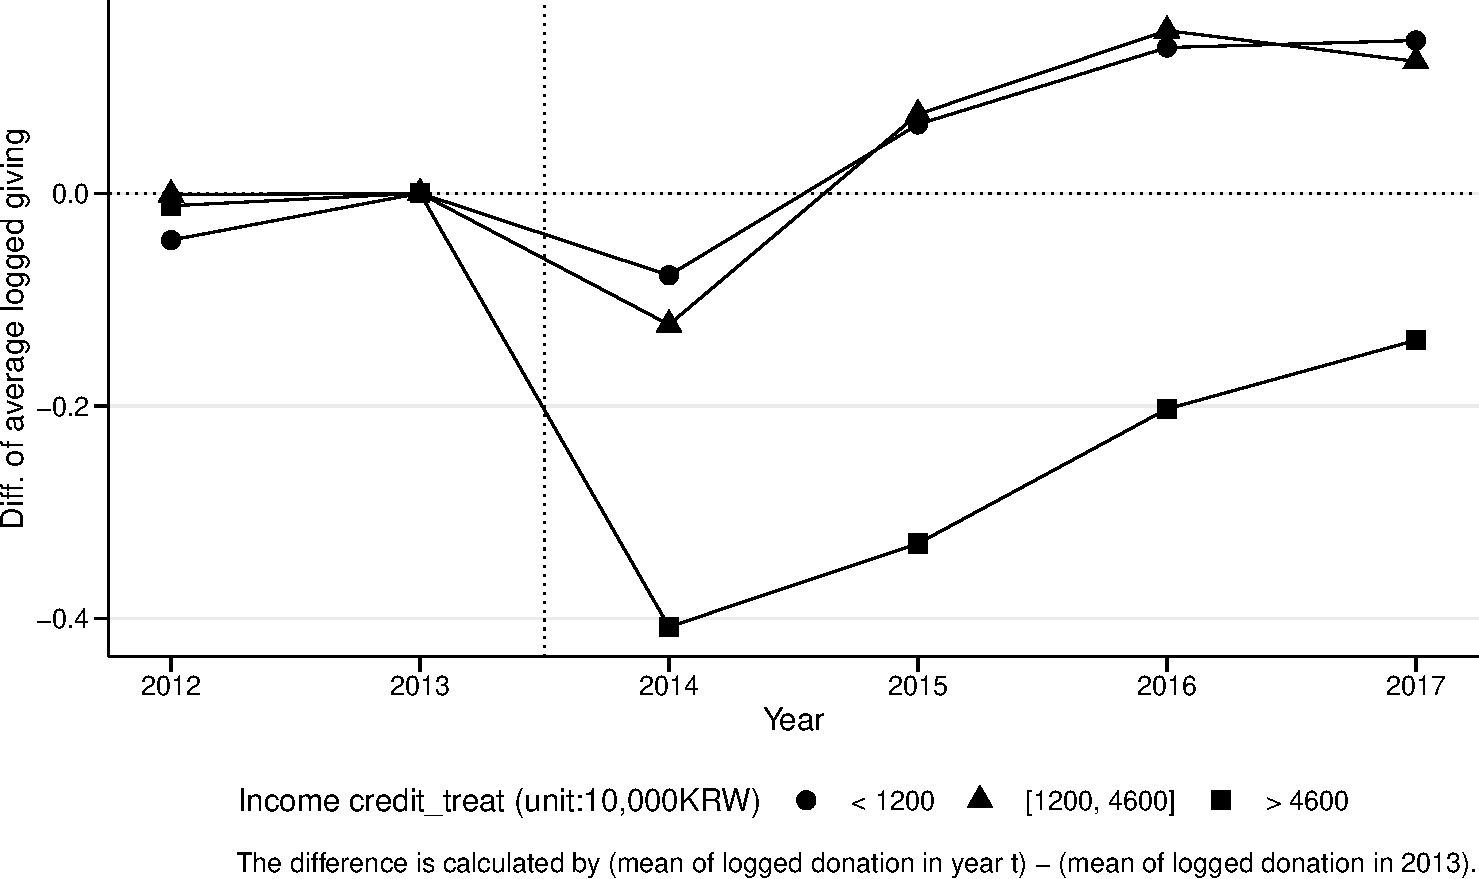
\includegraphics{C:/Users/vge00/Desktop/NASTAB/paper/draft_files/figure-latex/SummaryGivingOverall-1} 

}

\caption{Average Logged Giving by Three Income Groups. Notes: We created three income groups, with the relative price of giving rising (circle), unchanged (triangle), and falling (square) between 2013 and 2014. The group averages are normalized to be zero in 2013.}\label{fig:SummaryGivingOverall}
\end{figure}

図\ref{fig:SummaryGivingOverall}は
税インセンティブの変化に基づいた所得グループごとの平均寄付額を示している(非寄付者も含めている)。
この図から価格効果を観察できる。言い換えれば、税インセンティブは寄付行動を促進していることが観察される。
2015年以降、税制改革によって税インセンティブが拡大した(もしくは変化しなかった)人は所得控除時よりも増えているが、
税インセンティブが縮小した人は所得控除時よりも減少している。
また、寄付者に限定した平均寄付額と寄付者の割合のトレンドを所得グループごとに見ると、
似たような傾向が観察された
(補論\ref{addtab}の図\ref{fig:SummaryGivingIntensive}と図\ref{fig:SummaryGivingExtensive})。
ただし、寄付者に限定した平均寄付のトレンドを見ると、
図\ref{fig:SummaryGivingOverall}ほどはっきりとした価格効果を観察できない。

また、すべての所得グループの2014年の平均寄付額は2013年のそれを下回っている。
これはいくつかの可能性が考えられる。
第一に、税制改革のアナウンスメント効果である。
2014年の税制改革は2013年に告知されているので、
税インセンティブが縮小する所得グループにおいては、
2013年の寄付額を増やし、2014年の寄付額を減らすという異時点間の代替効果が予想される。
しかしながら、これは税インセンティブが拡大する所得グループの寄付額が減少した事実を説明できない。
第二の可能性は、制度の学習効果が考えられる。
税制改革直後は、税額控除によって自分が寄付によって節税しやすくなったかどうかが分からないので、
税インセンティブが拡大する所得グループでも寄付額は減少した。
それ以降、税インセンティブが拡大した納税者は自分が寄付によって節税しやすくなることを学習し、
寄付額を所得控除時よりも増やしたと考えられる。

寄付価格の変動は寄付控除の申告の有無でも生じる。
寄付控除を申告した場合の寄付の相対価格は図\ref{fig:SummaryPrice}に示した通りである一方で、
寄付控除を申告しない場合の寄付の相対価格は1である。
よって、控除の有無によって寄付の相対価格は変化する。
しかしながら、寄付控除の申告は自己選択なので、内生的である。
後に述べるように、この内生性を解決するために操作変数が必要である。

寄付控除の申告行動において、申告コストは大きな障害となっている可能性が高い。
補論\ref{addtab}の図\ref{fig:SummaryGivingIntensiveDist}に示しているように、
寄付控除の申告の有無によって、寄付者に限定した寄付額の分布は大きく変化しない。
これは寄付控除の申告の有無は、控除によって得られる便益の差よりも
申告するためのコストの差で説明できることを示唆している。

\begin{figure}[t]

{\centering 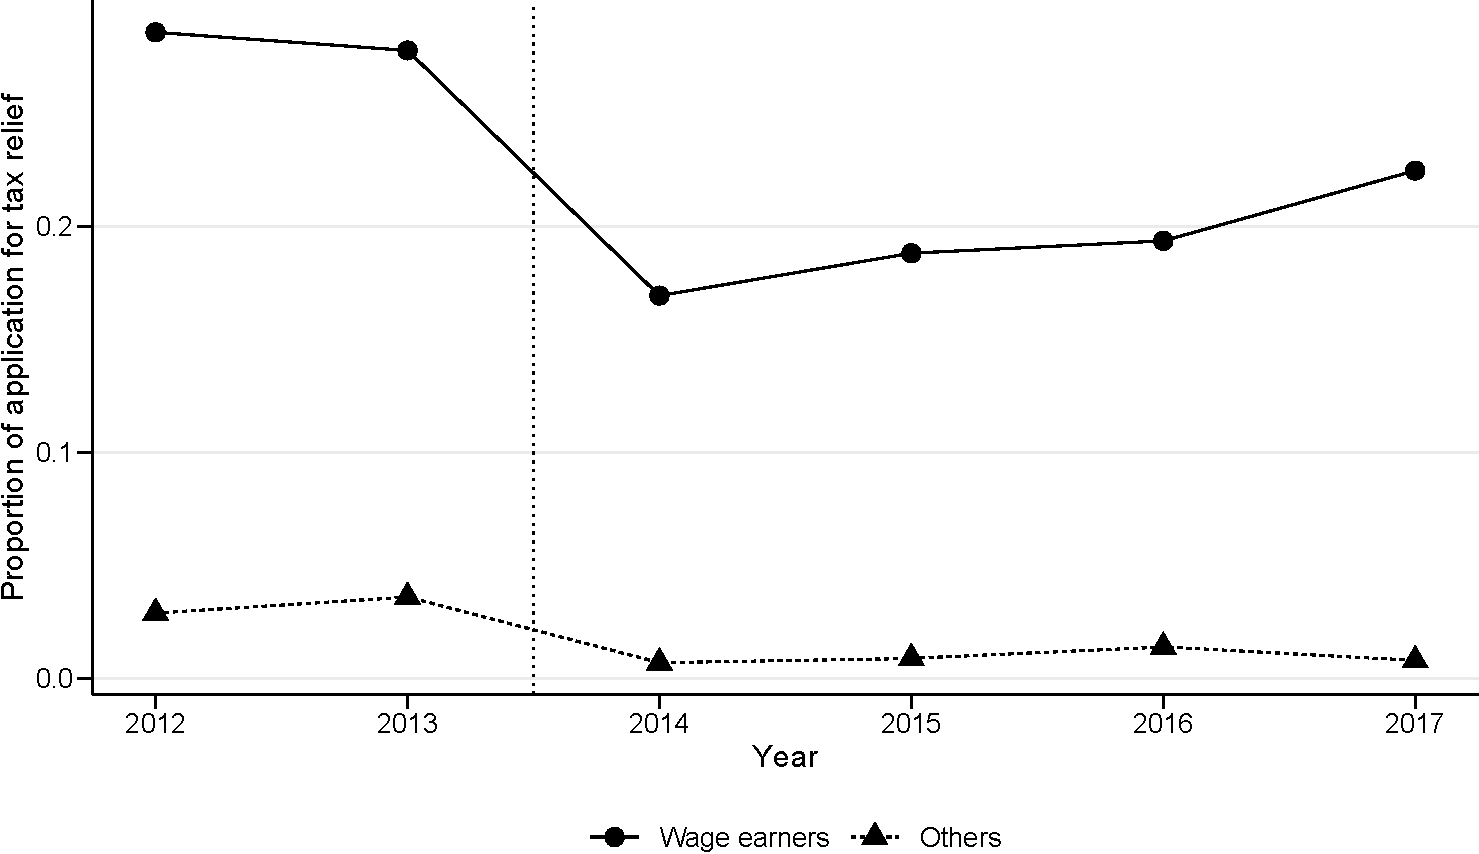
\includegraphics{C:/Users/vge00/Desktop/NASTAB/paper/draft_files/figure-latex/SummaryReliefbyEarner-1} 

}

\caption{Share of Tax Relief by Wage Earners. Notes: A solid line is the share of applying for tax relief among wage eaners. A dashed line is the share of applying for tax relief other than wage earners.}\label{fig:SummaryReliefbyEarner}
\end{figure}

以上を踏まえて、
我々は申告コストの要素の一つであるレコードキーピングに関する制度背景を第二の識別戦略として用いる。
先に述べたように、自営業者は寄付控除を申請するまで寄付の領収書(証明書)を保持しておく必要がある一方で、
給与所得者は会社を通じてその証明書をいつでも提出でき、
その後の申請も会社に手続きを依頼できる。
すなわち、給与所得者は自営業者よりも申告コストが低いことが予想される。
事実、図\ref{fig:SummaryReliefbyEarner}
給与所得者の控除の申請比率は自営業者よりもすべての期間を通じて高いことが分かる\footnote{寄付者に限定した控除の申告比率についても、給与所得者の方が自営業者よりも高い
  (補論\ref{addtab}の図\ref{fig:SummaryReliefbyEarner2})。}。
我々は給与所得者ダミーをレコードキーピングのコストの代理変数として操作変数に用いる。

\hypertarget{estimation}{%
\section{Empirical Strategy}\label{estimation}}

Almunia et al. (2020) に従い、我々は二種類の弾力性を推定する。
第一に、intensive-margin price elasiticityであり、
1\%の価格上昇で寄付者の寄付額が何\%増えるかを示している。
第二に、extensive-margin price elasiticityであり、
1\%の価格上昇で寄付者比率が何\%増えるかを示している。
第\ref{nastab}節で説明したように、
我々は2014年の税制改革による税インセンティブの変化を用いたDIDと
申告コストによる寄付控除の申請の有無を捉えた操作変数法の二つを組み合わせた識別戦略を用いる。

intensive-margin price elasticityは、
寄付者に限定して以下のtwo-way fixed effect modelを推定する。
\begin{align}
  \ln g_{it} = \theta_i + \gamma (R_{it} \times \ln (1 - s_{it}))
    + \beta X_{it} + \lambda_t + u_{it}, \label{eq:intensive}
\end{align}
ここで、\(X_{it}\)は課税前所得(\(y_{it}\))を含んだ共変量ベクトル、
\(\theta_i\)と\(\lambda_t\)はそれぞれ個人固定効果と時間固定効果である。
\(u_{it}\)はidiosyncratic errorである。
アウトカム変数\(\ln g_{it}\)は\(t\)年に寄付した人\(i\)の寄付額の対数値である。
寄付価格は\(R_{it} \times \ln (1 - s_{it})\)であり、
ここで、\(R_{it}\)は控除申請のダミー変数、\(s_{it}\)は税インセンティブである\footnote{寄付価格は\(\ln(1 - R_{it}s_{it})\)とも書ける。
  これは\(R_{it} \times \ln (1 - s_{it})\)と一致する。
  なぜなら、\(R_{it} = 0\)のとき、\(\ln(1) = 0\)となり、
  \(R_{it} = 1\)のとき、\(\ln(1 - s_{it})\)となる。}。
したがって、関心のあるパラメータは\(\gamma\)であり、
これがintensive-margin price elasticityを示す。

extensive-margin price elasticityの推定式は
two-way fixed effect付きの線形確率モデルである。
すなわち、
\begin{align}
  D_{it} = \theta_i + \delta (R_{it} \times \ln (1 - s_{it}))
    + \beta X_{it} + \lambda_t + \eta_{it}, \label{eq:extensive}
\end{align}
である。
アウトカム変数\(D_{it}\)は正の寄付額が観測されたら1を取るダミー変数である:\(D_{it} = 1[g_{it} > 0]\)。
ここで関心のあるパラメータは\(\delta\)である。
アウトカム変数は二値なので、このパラメータを弾力性として直接解釈できない。
extensive-margin price elasticityは\(\hat{\delta} / \bar{D}\)で得られる
(\(\bar{D}\)は\(D_{it}\)の標本平均)。

この推定式における二つの内生性に対する対処法について議論する。
第一に、
2014年の税制改革による税インセンティブの変化を寄付価格の外生的な変動要因として用いるが、
寄付価格の内生性は完全に排除できない。
寄付控除を申請した場合の寄付価格を以下のようになる。
\begin{align}
  1 - s_{it} =
  \begin{cases}
    1 - T'_t(y_{it} - g_{it})  \quad\text{if}\quad t < 2014  \\
    1 - m \quad\text{if}\quad t \ge 2014
  \end{cases},
\end{align}
ここで、\(T'_t(\cdot)\)は\(t\)年の限界所得税率、\(m\)は税額控除率(\(m = 0.15\))である。
寄付価格は2014年の税制改革だけではなく、
所得控除が適用される期間において、寄付額(\(g_{it}\))にも依存する。
これは\emph{last}-unit priceと呼ばれるものであり、この寄付価格は寄付額について内生的である\footnote{寄付額によるインセンティブの操作について、次の二つの可能性が考えられる。
  第一に、納税者は寄付額を減らすことで、所得税率を高められる(寄付価格を高められる)。
  第二に、納税者は寄付額を増やすことで、所得税率を下げられる(節税の額を増やせる)。}。

本研究は、過去の研究にならい、
last-unit priceの代わり(もしくはその操作変数)として\emph{first}-unit priceを用いる。
last-unit priceは最終的な寄付額で寄付価格を計算する一方で、
first-unit priceは寄付額をゼロとして寄付価格を計算する\footnote{first-unit priceは
  最初の1単位を寄付するかどうかの意思決定時に直面する価格として解釈できる。}。
すなわち、
\begin{align}
  1 - s^f_{it} =
  \begin{cases}
    1 - T'_t(y_{it} - 0)  \quad\text{if}\quad t < 2014  \\
    1 - m \quad\text{if}\quad t \ge 2014
  \end{cases}.
\end{align}
ただし、税額控除が適用される期間においては、
寄付価格が寄付額に依存しないので、last-unit priceとfirst-unit priceは一致する。

第二に、寄付控除申告の自己選択による内生性である。
申告コストがないとき、節税による便益を得られるので、
寄付者は全員寄付控除を申請するべきである。
しかしながら、我々のデータでは、寄付者の割合は24\%であるにも関わらず、
控除を申告した人の割合は10\%である(表\ref{tab:SummaryCovariate})。
また、補論\ref{addtab}の図\ref{fig:SummaryGivingIntensiveDist}に示しているように、
寄付控除の申告の有無によって、寄付者に限定した寄付額の分布は大きく変化しない。
これは寄付控除の申告行動において、申告コストは大きな障害となっている可能性が高いことを示唆している。

本研究はレコードキーピングの制度が給与所得者と自営業者で異なることを利用して、
給与所得者ダミー(\(WE_{it}\))をレコードキーピングのコストの代理変数として操作変数に用いる{[}\^{}exclusion{]}。
自営業者は寄付控除を申請するまで寄付の領収書(証明書)を保持しておく必要がある一方で、
給与所得者は会社を通じてその証明書をいつでも提出できるので、
給与所得者は自営業者よりも申告コストが低いことが予想される。

Wooldridge (2010) に従い、
我々は給与所得者ダミーを操作変数とした三つのアプローチを用いる\footnote{以降ではintensive-margin price elasticityの推定式を用いて説明するが、
  extensive-margin price elasticityの推定についても同じ方法が適用できる。}。
第一に、給与所得者ダミーとfirst-unit priceの交差項を
\(R_{it} \times \ln (1 - s^f_{it})\)の操作変数として用いる。
すなわち、intensive-margin price elasiticityの推定式は
\begin{align}
  \ln g_{it} = \theta_i + \gamma (R_{it} \times \ln (1 - s^f_{it}))
    + \beta X_{it} + \lambda_t + u_{it}, \label{eq:intensive2}
\end{align}
であり、
\(R_{it} \times \ln (1 - s^f_{it})\)の操作変数を\(WE_{it} \times \ln(1 - s^f_{it})\)とする\footnote{last-unit priceを用いて弾力性を推定する場合、
  \eqref{eq:intensive}もしくは\eqref{eq:extensive}の説明変数
  \(R_{it} \times \ln (1 - s_{it})\)の操作変数として
  \(WE_{it} \times \ln(1 - s^f_{it})\)を用いる。}。

残りの二つのアプローチは寄付申告の傾向スコアを用いるものである。
傾向スコアは以下のモデルをプロビット推定した予測確率で得られる。
\begin{align}
  R_{it} = 1[
    \alpha_0 + \alpha_1 WE_{it} + \alpha_2 \ln(1 - s^f_{it})
    + \alpha_3 X_{it} + u_{it0} > 0
  ] \label{eq:selection}
\end{align}

我々は全期間のサンプルを用いた推定(pooled model)と
年で分割したサブサンプルを用いた推定(separeted model)で傾向スコア\(\hat{P}_{it}\)を得た。
前者のモデルは式\eqref{eq:selection}の係数が時間に対して一定であると仮定している一方で、
後者のモデルは推定される係数が時間に依存することを許容したモデルである。

傾向スコアを用いた第二のアプローチは
式\eqref{eq:intensive2}の説明変数\(R_{it} \times \ln (1 - s^f_{it})\)の操作変数として
\(\hat{P}_{it} \times \ln (1 - s^f_{it})\)を用いる。
第三のアプローチは式\eqref{eq:intensive2}の説明変数\(R_{it} \times \ln (1 - s^f_{it})\)
の代わりに\(\hat{P}_{it} \times \ln (1 - s^f_{it})\)を用いる。すなわち、
我々は以下のモデルを推定する。
\begin{align}
  \ln g_{it} = \theta_i + \gamma (\hat{P}_{it} \times \ln (1 - s^f_{it}))
    + \beta X_{it} + \lambda_t + u_{it}, \label{eq:intensive3}
\end{align}

\hypertarget{result}{%
\section{Estimation Results}\label{result}}

\begin{table}

\caption{\label{tab:MainIntensive}Intensive-Margin Tax-Price Elasticity}
\centering
\fontsize{7}{9}\selectfont
\begin{threeparttable}
\begin{tabular}[t]{lcccccc}
\toprule
\multicolumn{1}{c}{ } & \multicolumn{3}{c}{FE} & \multicolumn{3}{c}{FE-2SLS} \\
\cmidrule(l{3pt}r{3pt}){2-4} \cmidrule(l{3pt}r{3pt}){5-7}
  & (1) & (2) & (3) & (4) & (5) & (6)\\
\midrule
Applying tax relief x log(first price) & \num{-0.748}*** &  &  & \num{-1.400}*** & \num{-1.437}*** & \num{-1.540}***\\
 & (\num{0.225}) &  &  & (\num{0.411}) & (\num{0.363}) & (\num{0.375})\\
PS of applying tax relief x log(first price) &  & \num{-1.544}*** & \num{-1.515}*** &  &  & \\
 &  & (\num{0.388}) & (\num{0.367}) &  &  & \\
\midrule
First-stage: Instrument &  &  &  & 0.638 & 1.075 & 0.984\\
 &  &  &  & {}[468.1] & {}[534.6] & {}[662.2]\\
Num.Obs. & \num{7004} & \num{6975} & \num{6975} & \num{6975} & \num{6975} & \num{6975}\\
Instrument &  &  &  & WE x Price & PS x Price & PS x Price\\
Method of PS &  & Pool & Separate &  & Pool & Separate\\
\bottomrule
\multicolumn{7}{l}{\rule{0pt}{1em}* p $<$ 0.1, ** p $<$ 0.05, *** p $<$ 0.01}\\
\end{tabular}
\begin{tablenotes}
\item Notes: $^{*}$ $p < 0.1$, $^{**}$ $p < 0.05$, $^{***}$ $p < 0.01$. Standard errors are clustered at individual level. A square bracket is wald statistics of instrument.
\end{tablenotes}
\end{threeparttable}
\end{table}

\hypertarget{ux7d50ux679c-extensive-margin-tax-price-elasticity}{%
\subsection{結果: Extensive-Margin Tax-Price Elasticity}\label{ux7d50ux679c-extensive-margin-tax-price-elasticity}}

\begin{table}

\caption{\label{tab:MainExtensive}Extensive-Margin Tax-Price Elasticity}
\centering
\fontsize{7}{9}\selectfont
\begin{threeparttable}
\begin{tabular}[t]{lcccccc}
\toprule
\multicolumn{1}{c}{ } & \multicolumn{3}{c}{FE} & \multicolumn{3}{c}{FE-2SLS} \\
\cmidrule(l{3pt}r{3pt}){2-4} \cmidrule(l{3pt}r{3pt}){5-7}
  & (1) & (2) & (3) & (4) & (5) & (6)\\
\midrule
Applying tax relief x log(first price) & \num{-2.800}*** &  &  & \num{-0.464}*** & \num{-0.563}*** & \num{-0.738}***\\
 & (\num{0.074}) &  &  & (\num{0.176}) & (\num{0.120}) & (\num{0.116})\\
PS of applying tax relief x log(first price) &  & \num{-0.452}*** & \num{-0.566}*** &  &  & \\
 &  & (\num{0.107}) & (\num{0.101}) &  &  & \\
\midrule
Implied price elasticity & -10.799*** & -1.741*** & -2.181*** & -1.788*** & -2.169*** & -2.841***\\
 & (0.287) & (0.411) & (0.388) & (0.678) & (0.463) & (0.448)\\
First-stage: Instrument &  &  &  & 0.289 & 0.803 & 0.768\\
 &  &  &  & {}[276.6] & {}[311.7] & {}[361.9]\\
Num.Obs. & \num{27017} & \num{26863} & \num{26863} & \num{26863} & \num{26863} & \num{26863}\\
Instrument &  &  &  & WE x Price & PS x Price & PS x Price\\
Method of PS &  & Pool & Separate &  & Pool & Separate\\
\bottomrule
\multicolumn{7}{l}{\rule{0pt}{1em}* p $<$ 0.1, ** p $<$ 0.05, *** p $<$ 0.01}\\
\end{tabular}
\begin{tablenotes}
\item Notes: $^{*}$ $p < 0.1$, $^{**}$ $p < 0.05$, $^{***}$ $p < 0.01$. Standard errors are clustered at individual level. A square bracket is wald statistics of instrument.
\end{tablenotes}
\end{threeparttable}
\end{table}

\hypertarget{ux30edux30d0ux30b9ux30c8ux30cdux30b9ux30c1ux30a7ux30c3ux30af}{%
\subsection{ロバストネスチェック}\label{ux30edux30d0ux30b9ux30c8ux30cdux30b9ux30c1ux30a7ux30c3ux30af}}

\begin{enumerate}
\def\labelenumi{\arabic{enumi}.}
\tightlist
\item
  2013-2014年データを除外 (Table \ref{tab:WoAnnoucementIntensive} and \ref{tab:WoAnnouncementExtensive})

  \begin{itemize}
  \tightlist
  \item
    税制改革のアナウンスメント効果を排除
  \end{itemize}
\item
  First-unit priceではなく、Last-unit priceで弾力性を推定 (Table \ref{tab:LastIntensive} and \ref{tab:LastExtensive})
\item
  給与所得者ダミーと寄付価格の交差項ではなく、first-unit priceを操作変数にする (Table \ref{tab:MainElasticity}-\ref{tab:WoAnnoucementElasticity})
\item
  寄付申告者に限定し、所得控除制度による内生性(e.g.~所得の変動)を考慮した分析を実施 (Table \ref{tab:R1Elasticity} and \ref{tab:KdiffElasticity})

  \begin{itemize}
  \tightlist
  \item
    階差モデルやリードラグ変数の使用 (Almunia et al., 2020; \textbf{Randolph1995?}; \textbf{Saez2002?})
  \end{itemize}
\end{enumerate}

ほとんどの分析で、intensive-margin tax-price elasticityは-1.5から-2の間に入り、
extensive-margin tax-price elasticityは-1.7から-5の間に入る

\hypertarget{ux97d3ux56fdux3067ux306eux5bc4ux4ed8ux306eux4fa1ux683cux5f3eux529bux6027ux306fux5148ux884cux7814ux7a76ux3088ux308aux5f3eux529bux7684}{%
\subsection{韓国での寄付の価格弾力性は先行研究より弾力的}\label{ux97d3ux56fdux3067ux306eux5bc4ux4ed8ux306eux4fa1ux683cux5f3eux529bux6027ux306fux5148ux884cux7814ux7a76ux3088ux308aux5f3eux529bux7684}}

\begin{itemize}
\tightlist
\item
  申告の自己選択を無視すると、Intensive-margin tax-price elasticityは過小推定

  \begin{itemize}
  \tightlist
  \item
    寄付者の寄付額を決める観察できない要素と申告が正の相関をしている
  \item
    そのような要素を寄付額を高めるならば、節税による便益が高くなるので、申告しやすくなる
  \end{itemize}
\item
  申告の自己選択を無視すると、Extensive-margin tax-price elasticityは過大推定

  \begin{itemize}
  \tightlist
  \item
    寄付価格が申告と寄付するかどうかの意思決定の両方に同じ方向の影響を与え、負の相関をより強くした可能性がある
  \end{itemize}
\end{itemize}

\hypertarget{conventional-method-to-estimate-tax-price-elasticity}{%
\subsection{Conventional Method to Estimate Tax-Price Elasticity}\label{conventional-method-to-estimate-tax-price-elasticity}}

\begin{table}

\caption{\label{tab:MainElasticity}Estimation of Last-Unit Price Elasticities}
\centering
\fontsize{7}{9}\selectfont
\begin{threeparttable}
\begin{tabular}[t]{lcccc}
\toprule
\multicolumn{1}{c}{ } & \multicolumn{2}{c}{Intensive margin} & \multicolumn{2}{c}{Extensive margin} \\
\cmidrule(l{3pt}r{3pt}){2-3} \cmidrule(l{3pt}r{3pt}){4-5}
\multicolumn{1}{c}{ } & \multicolumn{1}{c}{FE} & \multicolumn{1}{c}{FE-2SLS} & \multicolumn{1}{c}{FE} & \multicolumn{1}{c}{FE-2SLS} \\
\cmidrule(l{3pt}r{3pt}){2-2} \cmidrule(l{3pt}r{3pt}){3-3} \cmidrule(l{3pt}r{3pt}){4-4} \cmidrule(l{3pt}r{3pt}){5-5}
  & (1) & (2) & (3) & (4)\\
\midrule
log(last price) & \num{-0.634}*** & \num{-1.907}*** & \num{-2.945}*** & \num{-1.570}***\\
 & (\num{0.231}) & (\num{0.451}) & (\num{0.071}) & (\num{0.127})\\
\midrule
Implied price elasticity &  &  & -11.684*** & -6.227***\\
 &  &  & (0.281) & (0.502)\\
First-stage: log(first price) &  & 0.726 &  & 0.353\\
 &  & {}[442.4] &  & {}[407.8]\\
Num.Obs. & \num{7234} & \num{7234} & \num{28696} & \num{28696}\\
\bottomrule
\multicolumn{5}{l}{\rule{0pt}{1em}* p $<$ 0.1, ** p $<$ 0.05, *** p $<$ 0.01}\\
\end{tabular}
\begin{tablenotes}
\item Notes: $^{*}$ $p < 0.1$, $^{**}$ $p < 0.05$, $^{***}$ $p < 0.01$. Standard errors are clustered at individual level. A square bracket is wald statistics of instrument.
\end{tablenotes}
\end{threeparttable}
\end{table}

\hypertarget{conventional-method-to-estimate-tax-price-elasticity-2}{%
\subsection{Conventional Method to Estimate Tax-Price Elasticity (2)}\label{conventional-method-to-estimate-tax-price-elasticity-2}}

\begin{table}

\caption{\label{tab:WoAnnoucementElasticity}Estimation of Last-Unit Price Elasticities Excluding 2013 and 2014 data}
\centering
\fontsize{7}{9}\selectfont
\begin{threeparttable}
\begin{tabular}[t]{lcccc}
\toprule
\multicolumn{1}{c}{ } & \multicolumn{2}{c}{Intensive margin} & \multicolumn{2}{c}{Extensive margin} \\
\cmidrule(l{3pt}r{3pt}){2-3} \cmidrule(l{3pt}r{3pt}){4-5}
\multicolumn{1}{c}{ } & \multicolumn{1}{c}{FE} & \multicolumn{1}{c}{FE-2SLS} & \multicolumn{1}{c}{FE} & \multicolumn{1}{c}{FE-2SLS} \\
\cmidrule(l{3pt}r{3pt}){2-2} \cmidrule(l{3pt}r{3pt}){3-3} \cmidrule(l{3pt}r{3pt}){4-4} \cmidrule(l{3pt}r{3pt}){5-5}
  & (1) & (2) & (3) & (4)\\
\midrule
log(last price) & \num{-0.679}** & \num{-2.088}*** & \num{-3.097}*** & \num{-1.560}***\\
 & (\num{0.333}) & (\num{0.600}) & (\num{0.086}) & (\num{0.170})\\
\midrule
Implied price elasticity &  &  & -11.574*** & -5.830***\\
 &  &  & (0.320) & (0.634)\\
First-stage: log(first price) &  & 0.796 &  & 0.363\\
 &  & {}[270.6] &  & {}[244.3]\\
Num.Obs. & \num{5405} & \num{5405} & \num{20198} & \num{20198}\\
\bottomrule
\multicolumn{5}{l}{\rule{0pt}{1em}* p $<$ 0.1, ** p $<$ 0.05, *** p $<$ 0.01}\\
\end{tabular}
\begin{tablenotes}
\item Notes: $^{*}$ $p < 0.1$, $^{**}$ $p < 0.05$, $^{***}$ $p < 0.01$. Standard errors are clustered at individual level. A square bracket is wald statistics of instrument.
\end{tablenotes}
\end{threeparttable}
\end{table}

\hypertarget{estimating-price-elasticity-using-compliers}{%
\subsection{Estimating Price Elasticity Using Compliers}\label{estimating-price-elasticity-using-compliers}}

\begin{table}

\caption{\label{tab:R1Elasticity}Estimating Intensive-Margin Price Elasticities for Those Who Applied for Tax Relief}
\centering
\fontsize{5}{7}\selectfont
\begin{threeparttable}
\begin{tabular}[t]{lcccc}
\toprule
  & (1) & (2) & (3) & (4)\\
\midrule
log(first price) & \num{-1.203}*** & \num{-0.506} &  & \\
 & (\num{0.390}) & (\num{0.847}) &  & \\
log(last price) &  &  & \num{-1.330}*** & \num{-0.254}\\
 &  &  & (\num{0.452}) & (\num{0.903})\\
log(income) & \num{0.525} & \num{6.126} & \num{0.532} & \num{6.093}\\
 & (\num{0.776}) & (\num{5.365}) & (\num{0.785}) & (\num{5.503})\\
1-year lag of price &  & \num{0.369} &  & \num{0.487}\\
 &  & (\num{0.884}) &  & (\num{0.911})\\
1-year lag of income &  & \num{1.040} &  & \num{1.129}\\
 &  & (\num{4.777}) &  & (\num{5.030})\\
1-year lead of income &  & \num{-0.821} &  & \num{-0.826}\\
 &  & (\num{0.907}) &  & (\num{0.904})\\
\midrule
Instrument: log(first price) &  &  & 0.942 & -0.000\\
 &  &  & {}[3083.6] & {}[0.0]\\
Num.Obs. & \num{4079} & \num{1029} & \num{3972} & \num{1024}\\
\bottomrule
\multicolumn{5}{l}{\rule{0pt}{1em}* p $<$ 0.1, ** p $<$ 0.05, *** p $<$ 0.01}\\
\end{tabular}
\begin{tablenotes}
\item Notes: $^{*}$ $p < 0.1$, $^{**}$ $p < 0.05$, $^{***}$ $p < 0.01$. Standard errors are clustered at individual level. 1-year lead of price cannot be estimated because of collinearity.
\end{tablenotes}
\end{threeparttable}
\end{table}

\hypertarget{k-th-difference-model}{%
\subsection{\texorpdfstring{\(k\)-th Difference Model}{k-th Difference Model}}\label{k-th-difference-model}}

\begin{table}

\caption{\label{tab:KdiffElasticity}$k$-th Difference Model Using Those Who Applied for Tax Relief}
\centering
\fontsize{8}{10}\selectfont
\begin{threeparttable}
\begin{tabular}[t]{lccc}
\toprule
\multicolumn{1}{c}{ } & \multicolumn{1}{c}{1-year lag} & \multicolumn{1}{c}{2-year lag} & \multicolumn{1}{c}{3-year lag} \\
\cmidrule(l{3pt}r{3pt}){2-2} \cmidrule(l{3pt}r{3pt}){3-3} \cmidrule(l{3pt}r{3pt}){4-4}
  & (1) & (2) & (3)\\
\midrule
Difference of logged first price & \num{-1.890}* & \num{-2.530}*** & \num{-4.057}***\\
 & (\num{1.107}) & (\num{0.895}) & (\num{0.720})\\
\midrule
First-stage: Instrument & 0.995 & 0.991 & 0.984\\
 & {}[34401.5] & {}[31041.1] & {}[17987.3]\\
Num.Obs. & \num{4014} & \num{3903} & \num{3765}\\
Std.Errors & Clustered (pid) & Clustered (pid) & Clustered (pid)\\
FE: area & X & X & X\\
FE: indust & X & X & X\\
FE: year & X & X & X\\
\bottomrule
\multicolumn{4}{l}{\rule{0pt}{1em}* p $<$ 0.1, ** p $<$ 0.05, *** p $<$ 0.01}\\
\end{tabular}
\begin{tablenotes}
\item Notes: $^{*}$ $p < 0.1$, $^{**}$ $p < 0.05$, $^{***}$ $p < 0.01$. Standard errors are clustered at individual level. Instrument is difference between lagged first price in year $t$ and in year $t - k$ fixing income in year $t - k$.
\end{tablenotes}
\end{threeparttable}
\end{table}

\newpage

\hypertarget{appendix-appendix}{%
\appendix}


\hypertarget{addtab}{%
\section{Additional Tables and Figures}\label{addtab}}

\begin{figure}[H]

{\centering 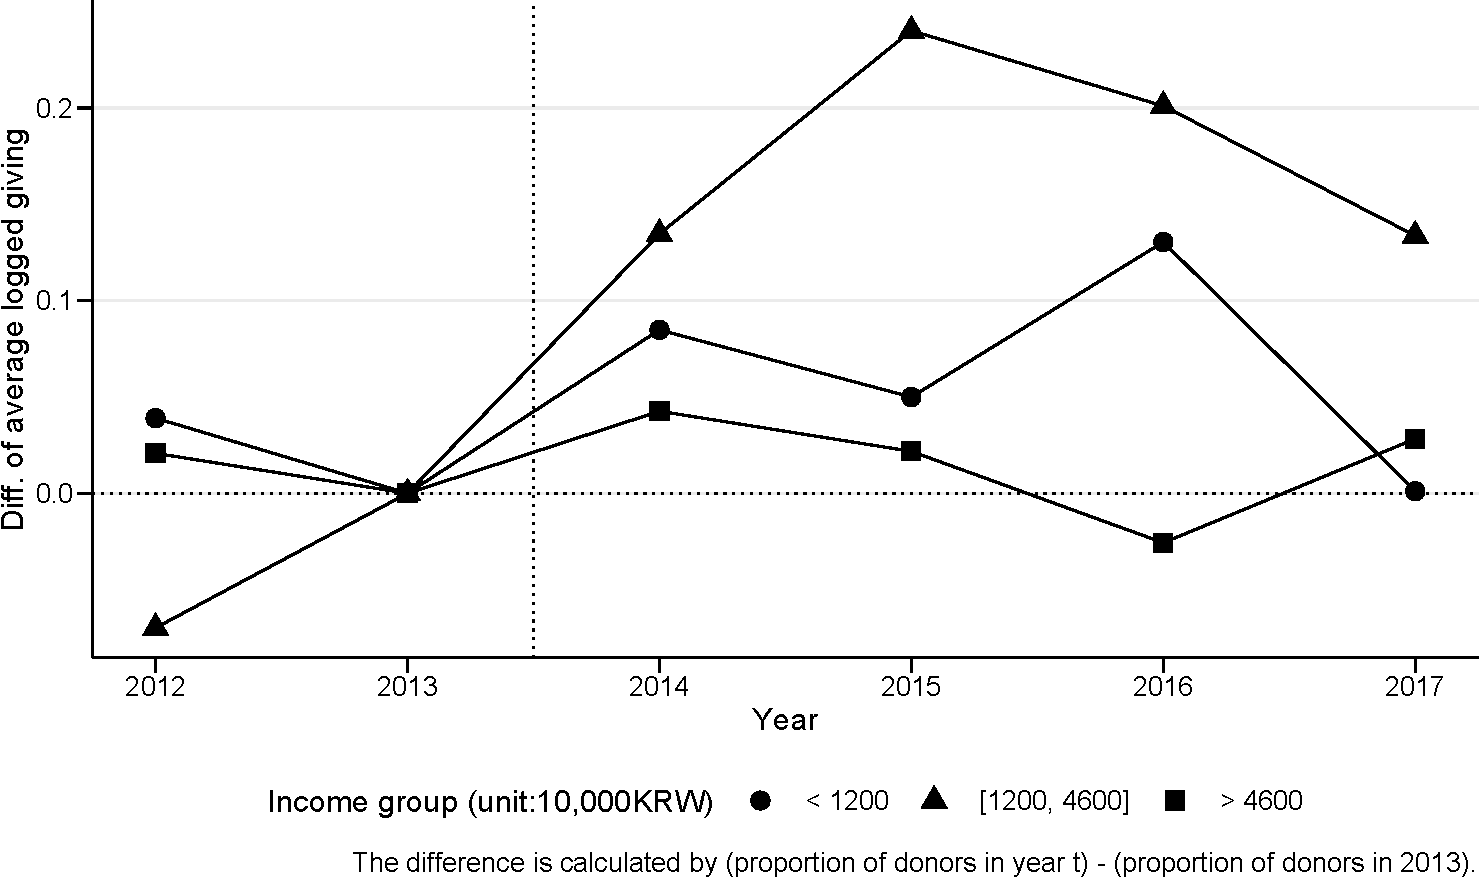
\includegraphics{C:/Users/vge00/Desktop/NASTAB/paper/draft_files/figure-latex/SummaryGivingIntensive-1} 

}

\caption{Average Logged Giving by Three Income Groups Conditional on Donors. Notes: We created three income groups, with the relative price of giving rising (circle), unchanged (triangle), and falling (square) between 2013 and 2014. The group averages are normalized to be zero in 2013.}\label{fig:SummaryGivingIntensive}
\end{figure}

\begin{figure}[t]

{\centering 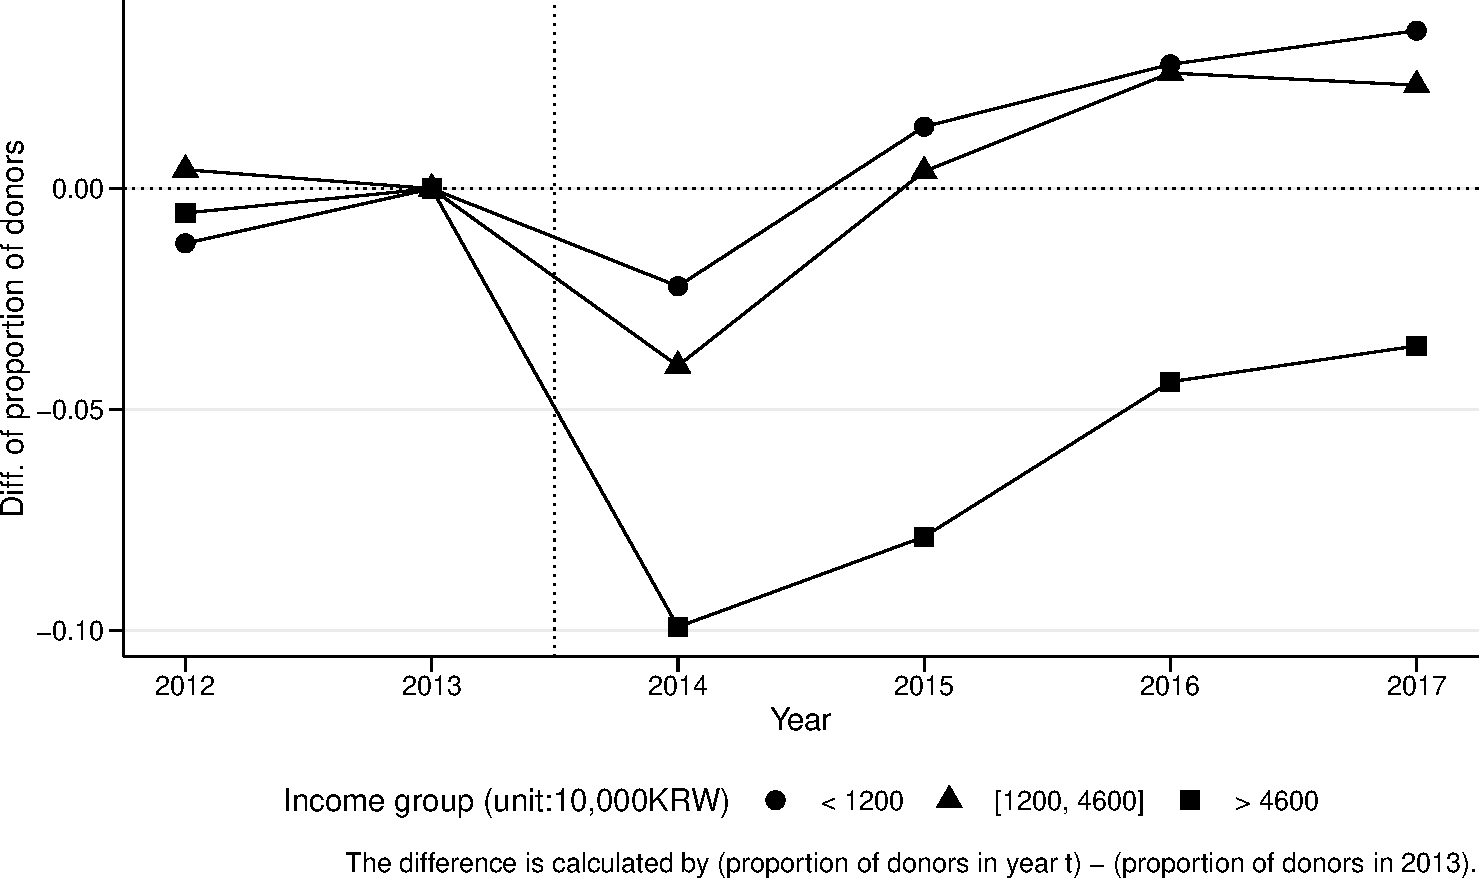
\includegraphics{C:/Users/vge00/Desktop/NASTAB/paper/draft_files/figure-latex/SummaryGivingExtensive-1} 

}

\caption{Proportion of Donors by Three Income Groups. Notes: We created three income groups, with the relative price of giving rising (circle), unchanged (triangle), and falling (square) between 2013 and 2014. The group averages are normalized to be zero in 2013.}\label{fig:SummaryGivingExtensive}
\end{figure}

\begin{figure}[t]

{\centering 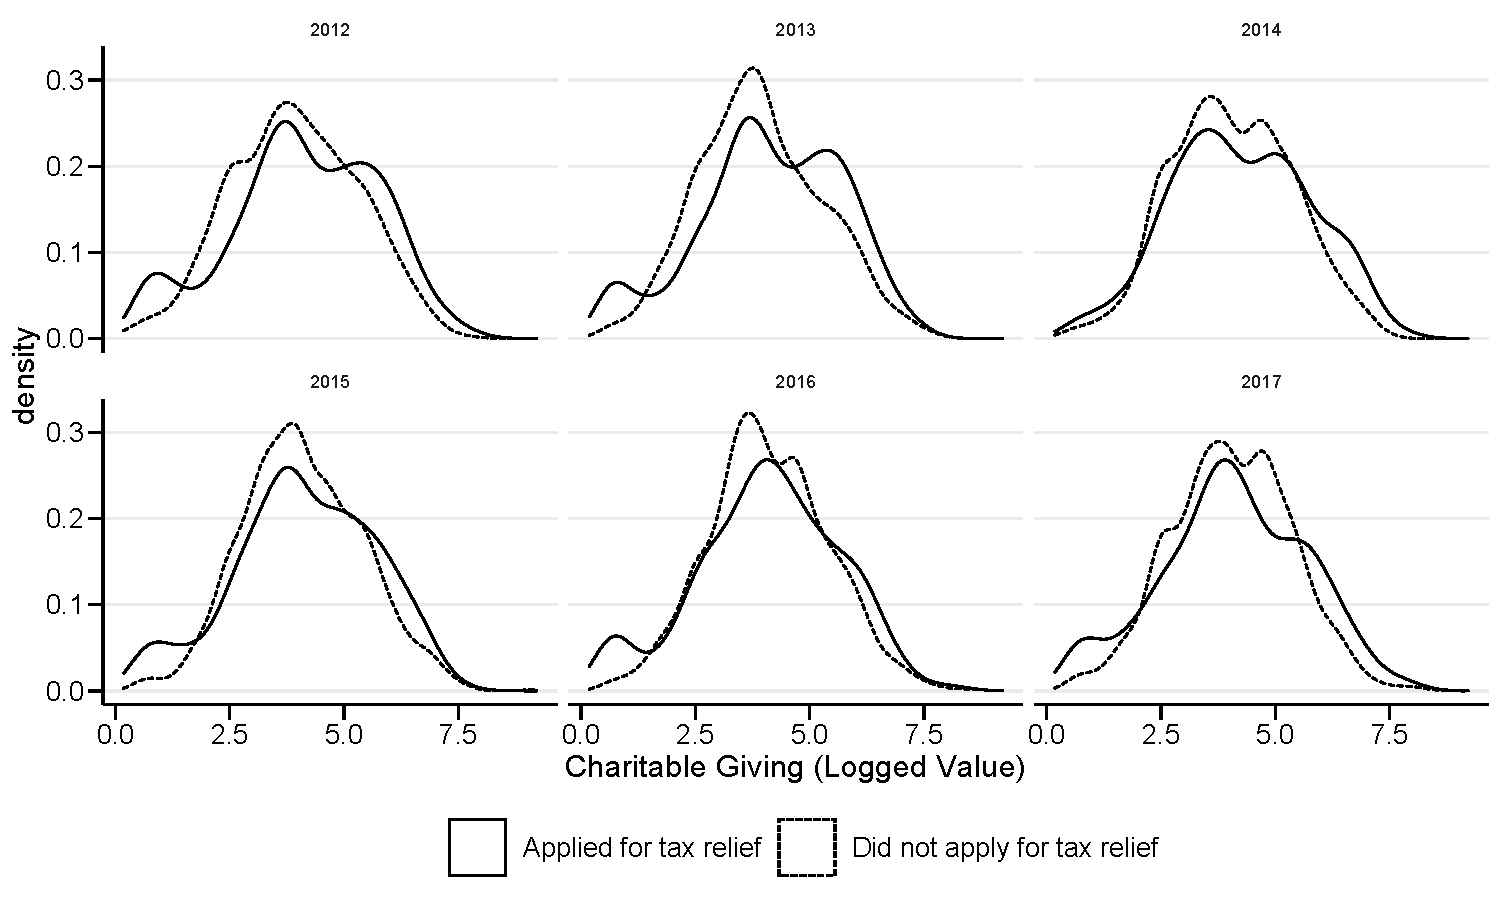
\includegraphics{C:/Users/vge00/Desktop/NASTAB/paper/draft_files/figure-latex/SummaryGivingIntensiveDist-1} 

}

\caption{Estimated Distribution of Charitable Giving among Donors in Each Year}\label{fig:SummaryGivingIntensiveDist}
\end{figure}

\begin{figure}[t]

{\centering 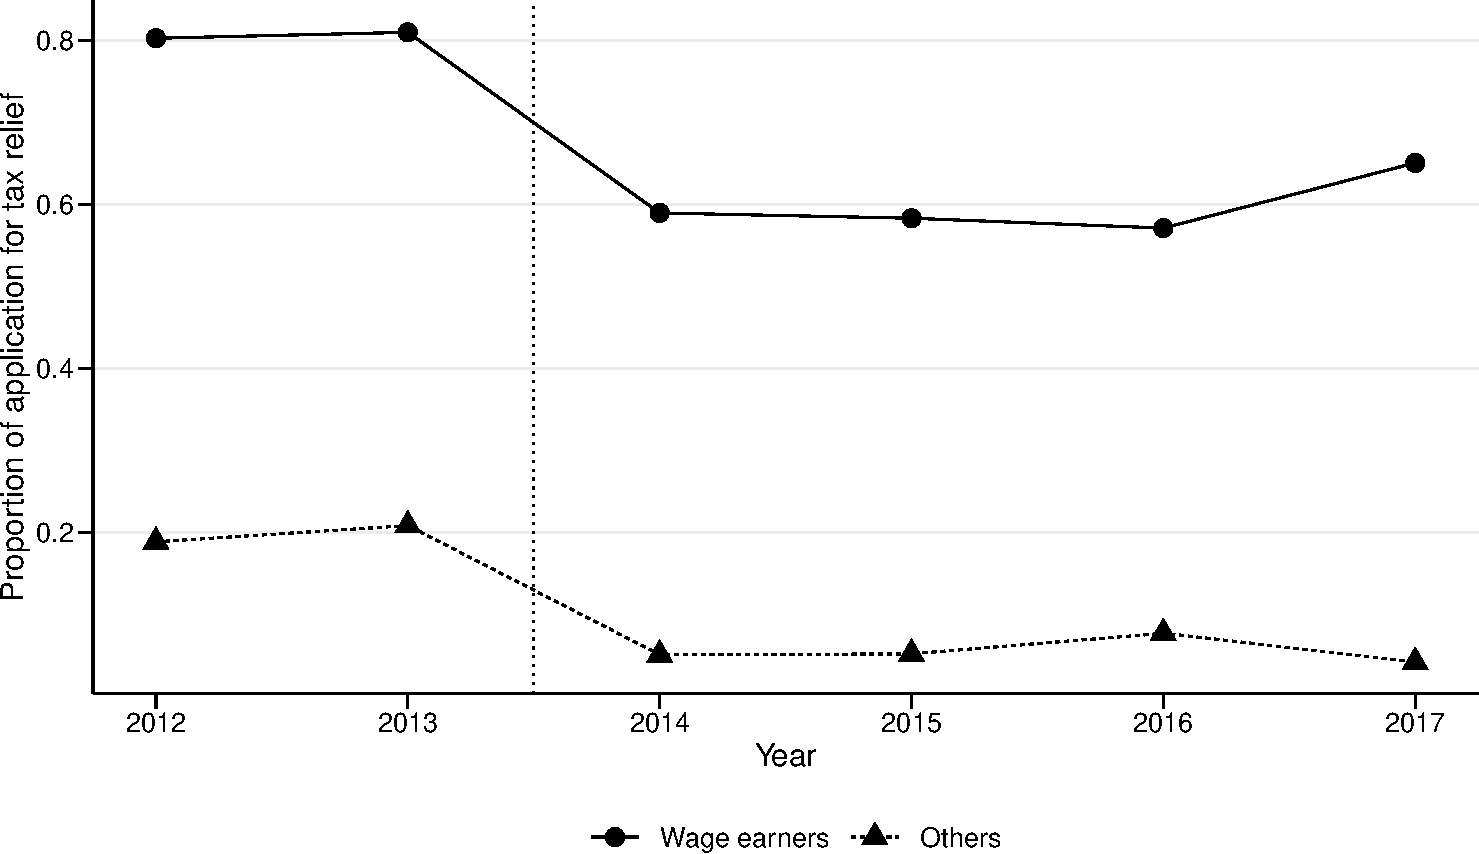
\includegraphics{C:/Users/vge00/Desktop/NASTAB/paper/draft_files/figure-latex/SummaryReliefbyEarner2-1} 

}

\caption{Share of Tax Relief by Wage Earners Conditional on Donors. Notes: A solid line is the share of applying for tax relief among wage eaners. A dashed line is the share of applying for tax relief other than wage earners.}\label{fig:SummaryReliefbyEarner2}
\end{figure}

\newpage

\hypertarget{references}{%
\section*{References}\label{references}}
\addcontentsline{toc}{section}{References}

\hypertarget{refs}{}
\begin{CSLReferences}{1}{0}
\leavevmode\vadjust pre{\hypertarget{ref-Scharf2020}{}}%
Almunia, M., Guceri, I., Lockwood, B., Scharf, K., 2020. More giving or more givers? {The} effects of tax incentives on charitable donations in the {UK}. Journal of Public Economics 183, 104114. doi:\href{https://doi.org/10.1016/j.jpubeco.2019.104114}{10.1016/j.jpubeco.2019.104114}

\leavevmode\vadjust pre{\hypertarget{ref-Wooldridge2010}{}}%
Wooldridge, J.M., 2010. Econometric analysis of cross section and panel data, 2nd ed. ed. {MIT Press}, {Cambridge, Mass}.

\end{CSLReferences}

\end{document}
